\appendix
\setcounter{figure}{0}
\renewcommand{\thefigure}{S\arabic{figure}}


\section{Likelihood of sample locations}
\label{appendix:MLE}

\textit{Notation}: For locations, we denote random variables by italicized uppercase letters, the values they take by the corresponding lowercase letters, and use asterisks to denote the observed values. Further, matrices are denoted by bold capital letters and parameters are denoted by greek letters. 

We start with assuming that the displacement along each edge of the ARG, $B_{edge}$, is independent. Hence each path, from a sample to the root, has an unique distribution for the location of the sample, even if they end at the same sample. We denote this set of locations by the $n_p$ length random vector, $\Lpvec$. In order to get the actual distribution of sample locations we condition on $\eta_{loops}$, i.e., we need to get the conditional probability density 
\begin{eqnarray}\label{eq:fLpLoops}
 f_{\Lpvec|\eta_{loops}}(\lpvec) = \frac{f_{\Lpvec}(\lpvec \cap \eta_{loops})}{f_{\Lpvec}(\eta_{loops})}. 
\end{eqnarray} 

However, we have that $\eta_{loops} = \eta_{paths}$ (appendix \ref{appendixC}). And since $\eta_{paths}$ is the condition that paths that end at the same samples have identical locations, the numerator becomes $f_{\Lpvec}(\lpvec \cap \eta_{loops}) = f_{\Lpvec}(\lpvec \cap \eta_{paths}) = f_{\Lpvec}(\Pp \lvec)$, where $\Pp$ is the path-sample matrix which is a $n_p \times n_s$ matrix whose $ij^{th}$ entry is 1 if the $i^{th}$ path ends at sample $j$ and $\lvec$ is a vector of length $n_s$ that has the location of each sample. 
Therefore, we have 
\begin{eqnarray}
\label{eqn:conditional}
    f_{\Lpvec|\eta_{loops}}(\lpvec) = \mathbb{1}[\lpvec = \Pp \lvec] \frac{f_{\Lpvec}(\Pp \lvec)}{f_{\Lpvec}(\eta_{paths})},
\end{eqnarray}
where $\mathbb{1}$ is the indicator function which is 1 if $\lpvec = \Pp \lvec$ and 0 otherwise. This basically ensures the probability density is 0 whenever any two paths ending at the same sample have different locations. We will now compute this distribution for the case of single root and then do the more general multiple root case. 

\subsection{Single Root}
For the case where the ARG has a single root, located at $\mu$, we have that the location of path ends, $\Lpvec$, is distributed multivariate normally with mean $\mu \onevec{{n_p}}$ and covariance matrix $\sigma^2 \spath$. Therefore, the numerator of Eq \ref{eqn:conditional},
\begin{eqnarray}
    \displaystyle f_{\Lpvec}(\Pp \lvec) 
  &=& \int \frac{1}{\sqrt{ (2\pi\sigma^2)^{\text{rnk }\spath} |\spath| }}\text{exp}\left( -\frac{(\lvec - \mu \onevec{{n_s}})^T \Pp^T\spathg\Pp (\lvec - \mu \onevec{{n_s}})}{2\sigma^2}\right)d\lvec.
\end{eqnarray}
We also evaluate the denominator in Eq \ref{eqn:conditional},
\begin{eqnarray}
  \displaystyle f_{\Lpvec}(\eta_{paths}) 
  &=& \int f_{\Lpvec}(\lpvec \cap \eta_{paths}) d\lpvec \\
  &=& \int f_{\Lpvec}(\Pp \lvec) d\lvec \\
  &=& \int \frac{1}{\sqrt{ (2\pi\sigma^2)^{\text{rnk }\spath} |\spath| }}\text{exp}\left( -\frac{(\lvec - \mu \onevec{{n_s}})^T \Pp^T\spathg\Pp (\lvec - \mu \onevec{{n_s}})}{2\sigma^2}\right)d\lvec \\
  &=& \frac{\sqrt{ (2\pi\sigma^2)^{n_s} |\mathbf{S}| }}{\sqrt{ (2\pi\sigma^2)^{\text{rnk }\spath} |\spath| }},
\end{eqnarray}
 where $\mathbf{S} = (\Pp^T\spathg\Pp)^{-1}$ is the sample covariance matrix.
 
 The probability density of the path locations, conditional on the loops (paths) meeting, is then
\begin{eqnarray}
    f_{\Lpvec|\eta_{loops}}(\lpvec) = \mathbb{1}[\lpvec = \Pp \lvec] \frac{1}{\sqrt{ (2\pi\sigma^2)^{n_s} |\mathbf{S}| }}\text{exp}\left( -\frac{(\lvec - \mu \onevec{{n_s}})^T \mathbf{S}^{-1}(\lvec - \mu \onevec{{n_s}})}{2\sigma^2}\right),
\end{eqnarray}
which is the probability density of a multivariate normal random variable with mean $\mu \onevec{{n_s}}$ and covariance matrix $\sigma^2\mathbf{S}$. This is the likelihood of sample locations, $\Lvec$, given Brownian motion down the ARG. The MLE of the dispersal rate and root location is then given by 
\begin{eqnarray}
\label{eqn:MLE}
    \widehat{\mu} &=& (\onevec{{n_p}}\spathg\onevec{{n_p}})^{-1}\onevec{{n_p}}\spathg\ldata \\
    \widehat{\sigma^2} &=& \frac{(\ldata - \mu\onevec{{n_s}})^T\Pp^T\spathg\Pp(\ldata - \mu\onevec{{n_s}})}{n_s}
\end{eqnarray}

\subsection{Multiple Roots}
\label{appendix:MultipleRoots}
We next want to generalize this to multiple roots, which occurs when we chop off an ARG at some time in the past. Let $n_r$ be the number of roots, $\muvec$ be $n_r \times 1$ vector of root locations, and $\Rp$ be the $n_p \times n_r$ path-root matrix defined in table \ref{table:methods}.
Then the probability distribution of the path locations is multivariate normal with mean $\Rp\muvec$ and covariance $\sigma^2\spath$.
Now, as in the single root case we want to find the  distribution of the path locations conditioned on the paths meeting at the samples (equation \ref{eq:fLpLoops}). 

As with a single root, the numerator can be written $f_{\Lpvec}(\lpvec \cap \eta_{loops}) = f_{\Lpvec}(\lpvec \cap \eta_{paths}) = f_{\Lpvec}(\Pp \lvec)$, but now this is
\begin{eqnarray}
\label{eq:numeration_multipleroots}
    f_{\Lpvec}(\Pp \lvec) = \frac{\exp[-\frac{1}{2\sigma^2}(\Pp \lvec - \Rp\muvec)^\trp\spathg(\Pp \lvec - \Rp\muvec)]}{\sqrt{(2\pi\sigma^2)^p|\spath|}}.
\end{eqnarray}
Similarly, the denominator becomes
\begin{eqnarray}
    f_{\Lpvec}(\eta_{paths}) &=& \displaystyle \int_{\bR^n} f_{\Lpvec} (\Pp \lvec) d\lvec \\
    &=& \displaystyle \int_{\bR^n} \frac{\exp[-\frac{1}{2\sigma^2}(\Pp \lvec - \Rp\muvec)^\trp\spathg(\Pp \lvec - \Rp\muvec)]}{\sqrt{(2\pi\sigma^2)^p|\spath|}}  d\lvec.
\end{eqnarray}
To find this integral we will multiply and divide by a constant to make the integrand a probability density for $\lvec$. In order to do that, note that the term in the exponent can be expanded like
\begin{eqnarray}
    && (\Pp \lvec - \Rp\muvec)^\trp\spathg(\Pp \lvec - \Rp\muvec) \\
    &=& \lvec^\trp \Pp^\trp \spathg \Pp \lvec - 2\muvec^\trp \Rp^\trp \spathg \Pp \lvec + \muvec^\trp \Rp^\trp \spathg\Rp \muvec \\
    &=& \lvec^\trp [\Pp, \Pp]\lvec - 2 \muvec^\trp {[\Rp,\Pp]}\lvec + \muvec^\trp [\Rp,\Rp]\muvec \\
    &=& \lvec^\trp [\Pp, \Pp]\lvec - 2 \muvec^\trp {[\Rp,\Pp]}[\Pp, \Pp]^{-1}[\Pp, \Pp]\lvec + \muvec^\trp [\Rp,\Rp]\muvec \\
    &=& \lvec^\trp [\Pp, \Pp]\lvec - 2 \muvec_\ell^\trp [\Pp, \Pp]\lvec + \muvec^\trp [\Rp,\Rp]\muvec \\
    &=& \lvec^\trp [\Pp, \Pp]\lvec - 2 \muvec_\ell^\trp [\Pp, \Pp]\lvec + \muvec_\ell^\trp [\Pp,\Pp]\muvec_\ell - \muvec_\ell^\trp [\Pp,\Pp]\muvec_\ell + ...\\ & & ...\ \muvec^\trp [\Rp,\Rp]\muvec\\
    &=& (\lvec - \muvec_\ell)^\trp [\Pp,\Pp] (\lvec - \muvec_\ell) -\muvec_\ell^\trp [\Pp,\Pp]\muvec_\ell + \muvec^\trp [\Rp,\Rp]\muvec \\
    &=& (\lvec - \muvec_\ell)^\trp [\Pp,\Pp] (\lvec - \muvec_\ell) +... \\ && ... \  \muvec^\trp \big([\Rp,\Rp] - {[\Rp,\Pp]}[\Pp, \Pp]^{-1}[\Pp,\Rp] \big) \muvec.
\end{eqnarray}
In step 1 above we have used $\lvec^\trp \Pp^\trp \spathg \Rp \muvec = \muvec^\trp \Rp^\trp \spathg \Pp \lvec$, as these are $1 \times 1$ matrices and therefore are the transpose of each other.
We have also used the shorthand $[\mathbf{A}, \mathbf{B}] = \mathbf{A}^\trp \spathg \mathbf{B}$ and introduced $\muvec_\ell = [\Pp, \Pp]^{-1}[\Pp,\Rp]\muvec $, a $n \times 1$ vector which will correspond to the expectation of the sample locations (as shown below).
Using this expansion, we have  
\begin{eqnarray}
    f_{\Lpvec}(\eta_{paths}) &=& N_{old} \displaystyle \int_{\bR^n} \exp\bigg[-\frac{1}{2\sigma^2}(\lvec - \muvec_\ell)^\trp [\Pp,\Pp] (\lvec - \muvec_\ell)\bigg]  d\lvec \\
    &=& N_{old} N_{new} \displaystyle \int_{\bR^n} \frac{\exp\bigg[\frac{-1}{2\sigma^2}(\lvec - \muvec_\ell)^\trp [\Pp,\Pp] (\lvec - \muvec_\ell)\bigg] }{\sqrt{(2\pi\sigma^2)^n|[\Pp,\Pp]^{-1}|}}  d\lvec \\
    &=& N_{old}N_{new}
\end{eqnarray}
where $\displaystyle N_{old} = \frac{\exp\bigg[ -\displaystyle\frac{1}{2\sigma^2}\muvec^\trp \big([\Rp,\Rp] - {[\Rp,\Pp]}[\Pp, \Pp]^{-1}[\Pp,\Rp] \big)\muvec\bigg]}{\sqrt{(2\pi\sigma^2)^p|\spath|}} $ and \\ $N_{new} = \sqrt{(2\pi\sigma^2)^n|[\Pp,\Pp]^{-1}|}$.

Using this notations, we can also rewrite Eq \ref{eq:numeration_multipleroots} as 
\begin{eqnarray}
    f_{\Lpvec}(\Pp \lvec) = N_{old} \exp\bigg[-\frac{1}{2\sigma^2}(\lvec - \muvec_\ell)^\trp [\Pp,\Pp] (\lvec - \muvec_\ell)\bigg]  
\end{eqnarray}

Dividing numerator by denominator, the distribution of the path locations after conditioning on the loops (paths) meeting is
\begin{eqnarray}
    f_{\Lpvec|\eta_{loops}}(\lpvec)
    &=& \frac{f_{\Lpvec}(\Pp \lvec \cap \eta_{paths})}{f_{\Lpvec}(\eta_{paths})} \\
    &=& \frac{N_{old} \exp\bigg[-\frac{1}{2\sigma^2}(\lvec - \muvec_\ell)^\trp [\Pp,\Pp] (\lvec - \muvec_\ell)\bigg]  }{N_{old}N_{new}} \\
    &=& \frac{ \exp\bigg[-\frac{1}{2\sigma^2}(\lvec - \muvec_\ell)^\trp [\Pp,\Pp] (\lvec - \muvec_\ell)\bigg]  }{N_{new}}
\end{eqnarray}
This is a multivariate normal distribution with mean $\muvec_\ell = [\Pp,\Pp]^{-1}[\Pp,\Rp]\muvec$ and covariance  $\sigma^2 \smat = \sigma^2 [\Pp,\Pp]^{-1}$. This is the likelihood of sample locations, $\Lvec$, given Brownian motion down the ARG.

\subsubsection{Maximum likelihood parameter estimates}
The log likelihood function for the parameters is then given by 
\begin{eqnarray}
    \log L(\muvec,\sigma^2) &=& -\frac{1}{2\sigma^2}(\lvec - \muvec_\ell)^\trp [\Pp,\Pp] (\lvec - \muvec_\ell) - n\log\sigma + const \\
    &=& -\frac{1}{2\sigma^2} \bigg[ \lvec^\trp [\Pp,\Pp] \lvec - 2 \muvec_\ell^\trp [\Pp, \Pp] \lvec + \muvec_\ell^\trp [\Pp,\Pp] \muvec_\ell \bigg] ... \\
    && ... -n\log \sigma + const. 
\end{eqnarray}

We can use this to find the MLE root locations by first differentiating the log likelihood function with respect to each root location
\begin{eqnarray}
    -2 \sigma^2\frac{\partial \log L}{\partial \mu_i} &=& -2 \frac{\partial \muvec_\ell^\trp}{\partial \mu_i}[\Pp,\Pp]\lvec + \frac{\partial \muvec_\ell^\trp [\Pp,\Pp] \muvec_\ell}{\partial \mu_i} \\
    &=& -2 \frac{\partial \muvec_\ell^\trp}{\partial \mu_i}[\Pp,\Pp]\lvec + \frac{\partial \muvec_\ell^\trp}{\partial \mu_i} [\Pp,\Pp] \muvec_\ell +  \muvec_\ell^\trp [\Pp,\Pp]\frac{\partial \muvec_\ell}{\partial \mu_i} \\
    &=& -2 \frac{\partial \muvec_\ell^\trp}{\partial \mu_i}[\Pp,\Pp]\lvec + 2\frac{\partial \muvec_\ell^\trp}{\partial \mu_i} [\Pp,\Pp] \muvec_\ell.
\end{eqnarray}
Now, note that since $\muvec_\ell = [\Pp, \Pp]^{-1}[\Pp,\Rp]\muvec$ then $\displaystyle \frac{\partial \muvec_\ell}{\partial \mu_i} = [\Pp, \Pp]^{-1}[\Pp,\Rp] \vec{e_i}$, where $\vec{e_i}$ is the unit vector of length $n$ with 1 in the $i^{th}$ position. Therefore, we have
\begin{eqnarray}
    -2 \sigma^2\frac{\partial \log L}{\partial \mu_i} &=& -2 \vec{e_i}^\trp [\Rp,\Pp]\lvec + 2 \vec{e_i}^\trp [\Rp,\Pp] [\Pp, \Pp]^{-1}[\Pp,\Rp]\muvec
\end{eqnarray}
Equating this to zero for all $i \in \{1,2,...,r\}$ we get the MLE root locations, $\widehat{\muvec}$, as the solutions to the following system of linear equations 
\begin{eqnarray}
    [\Rp,\Pp] [\Pp, \Pp]^{-1}[\Pp,\Rp]{\muvec} &=& [\Rp,\Pp]\lvec \\
    \Rightarrow \widehat{\muvec} &=& \big( [\Rp,\Pp] [\Pp, \Pp]^{-1}[\Pp,\Rp] \big)^{-1} [\Rp,\Pp]\ldata.
\end{eqnarray}

\begin{figure}[ht]
    \centering
    \includegraphics[width=\linewidth]{Images/SupplementaryFigures/MultipleRoots/RootLocationMethod.jpg}
    \caption{Root locations for two different ARG computed under the conditional and unconditional distributions. }
    \label{fig:RootLocationMethod}
\end{figure}

Note that using this equation to get the root locations leads to unexpected behaviour. Specifically, ancestor locations rapidly move away from each other as we go back in time (see Fig \ref{fig:RootLocationMethod}). This is probably because highest probability of two Brownian motions meeting, forwards in time, when they start at different locations is at the middle of their starting locations, which forces them to diverge backwards in time. To avoid this issue, we use the unconditional distribution of $\Lpvec$ (i.e., not conditioning on the paths meeting at the samples) to compute the MLE root locations, which gives 
\begin{eqnarray*} 
    \muvecMLE = (\Rp^\text{T}\spathg\Rp)^{-1} \Rp\spathg\Pp\ldata.
\end{eqnarray*}
This behaves as we expected, with ancestor locations that do not diverge (another panel of the figure we will put here). We leave a more complete understanding of why the conditioned distribution behaves unexpectedly to future work. Note that when there is a single root the conditional and unconditional MLE root locations are equal and collapse to the well-known MLE (Eq \ref{eqn:MLE}).

Differentiating the log likelihood function with respect to $\sigma^2$ and setting to zero, the MLE dispersal rate is
\begin{eqnarray}
    \widehat{\sigma^2} &=& \displaystyle \frac{(\ldata - \widehat{\muvec_\ell})^\trp \smat^{-1}(\ldata-\widehat{\muvec_\ell})}{n} \\ 
    &=& \displaystyle \frac{(\ldata - \widehat{\muvec_\ell})^\trp \Pp\spathg\Pp (\ldata-\widehat{\muvec_\ell})}{n}.
\end{eqnarray}


\section{Equivalence of Loops and Paths Methods}
\label{appendix:Equivalence}
Here we prove $\eta_{loops} = \eta_{paths}$ for any arbitrary ARG. Before providing a formal proof which requires more detailed notations, we outline the idea here. 

\begin{enumerate}
    \item In order to prove the equivalence, we need to show that for each condition in $\eta_{loops}$ there exists an equivalent condition or set of conditions in $\eta_{paths}$ and vice versa. In other words, for each loop we need to find a pair of paths that only differ inside that loop. And conversely, for every pair of paths from the same sample, we need to find a set of loops such that any difference in the paths belongs to one of the loops. 
    \item Given a loop, we find a pair of paths as follows
    \begin{enumerate}
        \item Find the bottom and top of the loop. This is where the loop begins and ends. 
        \item Find a path from the bottom to one of the samples. This exists because every node is connected to at least one sample.
        \item Find a path from the top to one of the roots. This exists because every node is connected to at least one root. 
        \item To get the two paths, insert a different path from the loop in between the two paths found in the above two steps. 
        \item These two paths now only differ in the edges contained in the loop.
    \end{enumerate}
    \item Given a pair of paths starting at the same sample, here is how you find the set of loops that are equivalent.
    \begin{enumerate}
        \item Start from the sample and move up one node at a time until you hit a node that is different in the two paths. This is the beginning of the first loop.
        \item Now, find the first node after the beginning of the first loop that is common to the two paths. This is the end of the first loop.
        \item If the two paths are identical after the end of the first loop, then we have found the equivalent loop condition. 
        \item If not, repeat the above steps starting from the end of the first loop to find the next loop and so on. Since all paths end at roots, this process will stop and we will have a set of loops that are equivalent to the pair of paths. 
    \end{enumerate}
    
\end{enumerate}


\subsection{Formal Notations}
\begin{definition}[Directed Graphs] \label{def:dgraphs} A directed Graph $G_d$ is a two-tuple, $(V,E_d)$ where $V$ is the finite set of vertices/nodes and $E_d \subseteq V \times V$ is the set of edges. 
\end{definition}
\begin{note}
$G_d$ is a directed graph so $(v,w) \in E_d$ does not necessarily imply $(w,v) \in E_d$. The edges are directed from the child node to the parent node.
\end{note}

\begin{definition}[Parents] Given a directed Graph $G_d = (V,E_d)$ and $v \in V$, par($v$) = $\{ w \in V : (v,w) \in E_d \}$ is the set of parent nodes of $v$ and ch($v$) = $\{ w \in V : (w,v) \in E_d \}$ is the set of child nodes of $v$. Further $|\text{par}(v)| $ and $|\text{ch}(v)|$ denote the number of parent nodes and child nodes of $v$
\end{definition}

\begin{definition}[Paths] Given a directed Graph $G_d = (V,E_d)$ and $v,w \in V$, a path from $v$ to $w$ is a sequence of vertices $p = (v_0,v_1,...,v_n)$ such that $(v_i,v_{i+1}) \in E_d$ $\forall \ i \in \{ 0,1,..,n-1 \} $ where $v_0= v $ and $v_n = w$. We will say $v$ is connected to $w$ if there exists a path from $v$ to $w$ and is denoted by $v \rightarrow w$. Further, we define for any $0 < l < m <n$, $p |_{v_l}^{v_m} = (v_l,v_{l+1},...,v_{m-1},v_m)$, the restriction of path $p$ between $v_l$ and $v_m$.


%\begin{note}
%    Note that we are thinking backwards in time. So successors are the parent nodes and the predecessors are the child nodes.
%\end{note}
    
\end{definition}

\begin{definition}[Loops] Given a directed graph $G_d$ and $v,w \in V$, we say there is a loop between $v$ and $w$ if there exists two paths, $\lambda_1 = (\lambda_{10},\lambda_{11},..,\lambda_{1n_1})$ and $\lambda_2 = (\lambda_{20},\lambda_{21},..,\lambda_{2n_2})$ from $v$ to $w$ such that $\lambda_{1i} \neq \lambda_{2j} \ \forall \ i \in \{1,2,..,n-1\}$ and $j \in \{ 1,2,...,n_2-1\}$, where $\lambda_{10}=\lambda_{20}=v$ and $\lambda_{1n_1}=\lambda_{2n}=w$. We will denote a loop by $\lambda = (\lambda_1,\lambda_2)$.
\end{definition}

\begin{definition}[Ancestral Recombination Graph] An Ancestral Recombination Graph (ARG) is a 4-tuple $(G_d, S, T, t)$, where $G_d = (V, E_d)$ is a directed graph, $S \subsetneq V$ is the set of samples, $T$ is the set of times, and $t: V \rightarrow T$ is a bijective function associating each node with its time such that 
\begin{enumerate}
    \item $(v,w) \in E_d \Rightarrow t(v) < t(w)$ 
    \item ch($s$) $= \varnothing \ \forall \ s \in S$ and $|ch(v)|>0 \ \forall \ v \notin S$
    \item $\exists \ w \in V $ such that $v \rightarrow w \ \forall \ v \in V$ and $t(v) < t(w)$. Such a $w$ is called a Grand Common Ancestor (GCA). Further the GCA with the least time is called the Grand Most Recent Common Ancestor (GMRCA). 
\end{enumerate}
Further, we say $v \in V$ is a recombination node if $|par(v)| = 2$ and $v$ is said to be a coalescence node if $|ch(v)| > 1$. $4(a)$ is necessary since an individual cannot have more than 2 parents. $4(b)$ ensures that there are no multiple merger nodes but is not necessary. $4(c)$ ensures that a node is not both a recombination node and a coalescence node. 
\end{definition}

\subsection{Spatial Ancestral Recombination Graphs (SpARGs)}

\begin{definition}[SpARG] A d-dimensional Spatial Ancestral Recombination Graph $SpARG$ is an ARG with a set of locations $L \subset \mathbb{R}^d $ and a bijective function $l:V \rightarrow L$ which maps each vertex to its spatial location. 
\end{definition}
$\rightarrow$ \\
We are interested in estimating the dispersal rate given a particular SpARG under a model of Brownian motion. Therefore, we assume that displacement along any given edge of an ARG is determined by an independent Brownian motion. However, in order to get the ARG, these independent motions need to satisfy certain conditions. Essentially, we need to condition on these independent Brownian motions forming the loops present in the ARG. For this we build a few more notations and definitions. \\ \\ 
% Let, $\mathbf{}$
For any edge $(v,w) \in E_d$, let $B_{vw} \sim \mathcal{N}( 0, \sigma^2 t_{vw})$ be the distribution of the displacement along that edge under Brownian motion where $t_{vw} = t_w - t_v$. We then define the displacement function that takes a path as an input and returns the displacement
\begin{eqnarray*}
D : P &\rightarrow& \mathbb{R} \\
p = (v_i)_{i=0}^{k} &\mapsto& \sum_{i=0}^{k-1} B_{v_iv_{i+1}}
\end{eqnarray*}
In order for these independent Brownian motions to be consistent with the ARG, they need to form the loops present. Let the conditions required for this be
\begin{eqnarray*}
    \eta_{loops} &=& \{ \displaystyle \sum_{i=0}^{n-1} B_{v_i v_{i+1} } = \sum_{i=0}^{m-1} B_{w_i w_{i+1} } : \big( (v_i)_{i=0}^{n}, (w_i)_{i=0}^{m} \big) \text{ is a loop between $v$ and $w$ in $ARG_{sp}$ }    \}
\end{eqnarray*}
This ensures that the Brownian motions meet in a way that they form the loops in the ARG. 
Now, let $X_i$ denote the displacement of the $i^{th}$ sample in $S$, $s_i$, relative to the GMRCA. Then the probability distribution of $\mathbf{X} = \{ X_i \}_{i=1}^{n}$, where $n = |S|$ is the number of samples, is given by 
\begin{eqnarray}
    \label{Eq:pdist}
    P_\mathbf{X}(x_1,x_2,..,x_n) = p_\mathbf{B}(x_1,x_2,..,x_n | \eta_{loops})
\end{eqnarray}
 where $B_i = \displaystyle D(p_i)$ is the displacement along a path $p_i = ( s_{ij})_{j=0}^{n_i}$ from $s_i$ to the GMRCA. Note that for Eq \ref{Eq:pdist} to be well-defined, that is for it have a unique value for a given set of input positions, the value should not depend on the choice of the path from a sample to the GMRCA. To define this more formally, let $P_i = \{ (s_{ij} )_{j=0}^{n_i} : s_{i0} = s_i, s_{in_i} = v_{GM}, (s_{ij},v_{i,j+1}) \in E_d \ \forall \ 0\leq j < n_i  \}$ be the set of paths from $s_i$ to the GMRCA. Now, 
\begin{eqnarray*}
    \eta_{i, paths} &=& \{ \displaystyle D(p_{i1}) = D(p_{i2}): p_{i1}, p_{i2} \in P_i     \} \\
    \eta_{paths} &=& \displaystyle \bigcup_{i=1}^{n} \eta_{i,paths} 
\end{eqnarray*}

Now, as long as $\eta_{paths}$ is true Eq \ref{Eq:pdist} is well-defined. We will show that $\eta_{loops} = \eta_{paths}$ which would do the trick. 
 
\begin{lemma} $\eta_{paths} = \eta_{loops}$ 
\end{lemma}
\begin{proof}
[$\Rightarrow$] We will first show that $\eta_{paths} \subseteq \eta_{loops} $. Therefore, we need to show that given any two paths $p_{i1} = (s_{ij}^{(1) } )_{j=0}^{n_i^{(1)}}$ and $p_{i2} = (s_{ij}^{(2)} )_{j=0}^{n_i^{(2)}}$ between a sample, $s_i$, and the GMRCA, there exists loops $\lambda^{(1)},\lambda^{(2)},...,\lambda^{(m)}$ such that 
\begin{eqnarray*}
    \displaystyle \sum_{j=0}^{n_1^{(l)}-1} B_{\lambda_{1j}^{(l)} \lambda_{1,j+1}^{(l)} } = \sum_{j=0}^{n_2^{(l)}-1} B_{\lambda_{2j}^{(l)} \lambda_{2,j+1}^{(l)} } \ \forall \ 1 \leq l \leq m \Leftrightarrow \sum_{j=0}^{n_i^{(1)}-1} B_{s_{ij}^{(1)}  s_{i,j+1}^{(k_1)} } = \sum_{j=0}^{n_i^{(2)}-1} B_{s_{ij}^{(2)}  s_{i,j+1}^{(k_2)} }
\end{eqnarray*}
Here is how to find the loops starting from the two distinct paths. Let $n_{min} = \text{min}\{ n_i^{(1)},n_i^{(2)} \}$ and $n_{max} = \text{max}\{ n_i^{(1)},n_i^{(2)} \} $. Then define $J := \{ j \in \{0,1,...,n_{min} \} : s_{il}^{(k_1)} = s_{il}^{(k_2)} \ \forall \ l \leq j \}$ and $j_{st} := \text{max}J $. Now, $j_{st} < n_{max}$, otherwise we will have that $s_{il}^{(k_1)} = s_{il}^{(k_2)} $ for all $l$, which would mean the two paths are identical leading to a contradiction since we started with two distinct paths. Therefore,
\begin{eqnarray*}
    j_{st} < n_{max}.
\end{eqnarray*}
Let $v_{st}^{(1)} = s_{ij_{st}}^{(1)} = s_{ij_{st}}^{(2)} $. This is the start of the first loop. To find the end of this loop, let $V_{end} := \{ u \in p_{i1} \cap p_{i2} : t_u > t_{v_{st}^{(1)}} \} $. Then, $v_{end}^{(1)} = \displaystyle \min_{t(u)} V_{end} $. Note that $\lambda_1 = ( p_{i1}|_{v_{st}^{(1)}}^{v_{end}^{(1)}}, p_{i2}|_{v_{st}^{(1)}}^{v_{end}^{(1)}})$ is a loop. \\ \\ 
Now, if $p_{i1} |_{v_{end}^{(1)}}^{v_{GM}} = p_{i2} |_{v_{end}^{(1)}}^{v_{GM}} $, then we are done. Since everything before $v_{st}^{(1)}$ and after $v_{end}^{(1)}$ are identical in the two paths, the displacement along the two paths being equal is the same as the displacements forming the loop $\lambda_1$. \\ \\
If $p_{i1} |_{v_{end}^{(1)}}^{v_{GM}} \neq p_{i2} |_{v_{end}^{(1)}}^{v_{GM}} $, then we can repeat the above steps on $p_{i1} |_{v_{end}^{(1)}}^{v_{GM}}$ and $p_{i2} |_{v_{end}^{(1)}}^{v_{GM}}$, to find $v_{st}^{(2)}$ and $v_{end}^{(2)}$ such that $\lambda_2 = ( p_{i1}|_{v_{st}^{(2)}}^{v_{end}^{(2)}}, p_{i2}|_{v_{st}^{(2)}}^{v_{end}^{(2)}})$ is a loop and $p_{i1} |_{v_{end}^{(1)}}^{v_{st}^{(2)}} = p_{i2} |_{v_{end}^{(1)}}^{v_{st}^{(2)}} $. Keep repeating this until we have $(v_{st}^{(k)}, v_{end}^{(k)})_{k=1}^m$ such that $\lambda_l = ( p_{i1}|_{v_{st}^{(l)}}^{v_{end}^{(l)}}, p_{i2}|_{v_{st}^{(l)}}^{v_{end}^{(l)}}) $ are loops and $p_{i1} |_{v_{end}^{(l)}}^{v_{st}^{(l+1)}} = p_{i2} |_{v_{end}^{(l)}}^{v_{st}^{(l+1)}} \ \forall \ 1 \leq l \leq m$ where $v_{st}^{(m+1)} = v_{GM}$. We can do this because it is a finite graph. \\ \\
Therefore, the displacement along the two parts being equal is equivalent to the displacements forming the loops $\lambda_1, \lambda_2,..,\lambda_m$. \\
Thus, $\eta_{paths} \subseteq \eta_{loops}$. \newline
[$\Rightarrow$] Now we will show that $\eta_{loops} \subseteq \eta_{paths}$. That is we need to show that given a loop $\lambda$, there exists a pair of paths $p_{i1}$ and $p_{i2}$ from a sample to the GMRCA such that 
\begin{eqnarray*}
    \displaystyle \sum_{j=0}^{n_i^{(k_1)}-1} B_{s_{ij}^{(1)}  s_{i,j+1}^{(1)} } = \sum_{j=0}^{n_i^{(2)}-1} B_{s_{ij}^{(2)}  s_{i,j+1}^{(2)} } \Rightarrow \sum_{j=0}^{n_1-1} B_{\lambda_{1j} \lambda_{1,j+1} } = \sum_{j=0}^{n_2-1} B_{\lambda_{2j} \lambda_{2,j+1} } 
\end{eqnarray*}
Here is how you find two distinct paths given a loop $\lambda$. Suppose $\lambda$ is a loop from $v$ to $w$. By definition of an ARG, $w \rightarrow v_{GM}$. Let this path be $p_{wv_{GM}}$ \\ \\
Now, if $v \in S$, then $p_{i1} = \lambda_1 \cup p_{wv_{GM}}$ and $p_{i2} = \lambda_2 \cup p_{wv_{GM}}$ are two distinct paths from the sample $v$ to the GMRCA $v_{GM}$. Therefore, the condition for the Brownian motions to form the loop $\lambda_1$ is the same as the displacement along $p_{i1}$ being equal to $p_{i2}$. \\ \\
Now, if $v \notin S$, then we claim that there exists a sample $s_i \in S$ such that $s_i \rightarrow v$. Suppose not, i.e., $s_i \nrightarrow v \ \forall \ 1 \leq i \leq n $. Since $v \notin S$, therefore $\exists v^{(1)}$ such that $(v^{(1)},v) \in E_d$ by definition of an ARG. Now $v^{(1)}$ also does not belong to $S$, otherwise we will have a vertex in $S$ that is connected to $v$. Similarly, by induction we can construct $\{ v^{(k)} \}_{k \in \mathbb{N}}$ such that $(v^{(k)},v^{(k+1)}) \in E_d$ and $v^{(k)} \notin S \ \forall \ k \in \mathbb{N}$.  Therefore we have infinite vertices in the $ARG$ which is a contradiction. Therefore our claim has to be true. Let the path between $s_i$ and $v$ be $p_{iv}$, then $p_{iv} \cup \lambda_1 \cup p_{wv_{GM}}$ and $p_{iv} \cup \lambda_2 \cup p_{wv_{GM}}$ are the two required paths. Therfore, $\eta_{loops} \subseteq \eta_{paths}$ \\ \\ 
Therefore, we have that $\eta_{loops} = \eta_{paths}$ .
\end{proof}

\section{Minimal Path Matrix}
\label{appendixC:description}
Note that $\eta_{loops}$ will have exactly as many conditions as the number of recombination nodes, say $k$, in the ARG. However, the size of the full paths matrix is $n_p$, the total number of paths, which is strictly greater than $2*k + n_s$ and is bounded above by $2^k n_s$. Consequently, the number of conditions in $\eta_{paths}$ is bounded by $\displaystyle \binom{n_p}{2}$, which increases at least quadratically in $k$ and potentially exponentially. Therefore, $\eta_{paths}$ has multiple redundant conditions. But we only need one pair of paths for each condition $\eta_{loops}$, which only differ in one loop. We further need atleast one path each sample. Therefore, if chosen correctly, we only need $n_s + k$ paths to get the correct estimates. We call the matrix of shared times of these $n_s + k$ paths as the minimal path matrix.

Though there are existing methods in {\tt Python} (using the {\tt all\_simple\_paths()} function of {\tt networkx} package ) to identify all paths from the samples to the roots, calculating the intersection between these paths does not scale well to larger ARGs, primarily due to repeated calculation of common edges across different paths. We therefore developed an algorithm, outlined below, that requires traversing each edge only once and, in doing so, have greatly sped up the calculation of $\spath$. 

Briefly, the algorithm entails a bottom-up traversal of the ARG starting at the sample nodes and updating the shared time matrix as we move upwards towards the roots (Figure \ref{fig:algo_and_bench}). For each node visited, the algorithm calculates the edge length between that node and its parent. This is added to the corresponding cells in the shared time matrix. When we reach a recombination node (which has multiple parents), the relevant rows and columns are duplicated, expanding the size of the matrix and corresponding with the separation of these paths in the ARG. This keeps the size of the matrix small for as long as possible, making it more efficient. Currently, the algorithm is implemented using the {\tt tskit} package \citep{Kelleher2018}.


\subsection{Algorithm (step by step)}
\label{appendixC}

\begin{figure}[h!]
    \centering
    \includegraphics[width=0.75\linewidth]{Images/SupplementaryFigures/Algorithm/Benchmark.png}
    
    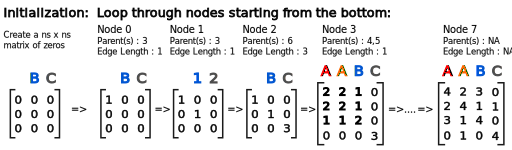
\includegraphics[width=\linewidth]{Images/SupplementaryFigures/Algorithm/AlgorithmExample.png}
    \caption{\textbf{Algorithm benchmarks}. Number of seconds to compute the full path and minimal path matrices using different algorithms plotted as a function of the total number of paths in the ARG. "Full Path Matrix - Naive" (blue) uses existing Python methods to compute the full path matrix. "Full Path Matrix - Bottom up" (red) instead computes the full path matrix with a single bottom-up traversal of the ARG. ``Minimal Path Matrix" (orange) uses the bottom-up method to compute the covariance between the smallest set of linearly independent paths, which is sufficient for estimating parameters of interest. Random ARGs of various sizes were generated (number of samples ranged up to 500 and sequence lengths up to 5000 basepairs) using the msprime Python package. The solid lines are the best fits under a power law. The best fit exponents for the power law are 2.946 (Full Path - Naive), 1.432 (Full Path - Bottom up) and 0.853 (Minimal Path).}
    \label{fig:algo_and_bench}
\end{figure}

\begin{enumerate}
    \item Initialization 
    \begin{itemize}
        \item The shared time matrix $\mathbf{S} \leftarrow [0]_{n \times n}$, a zero square matrix of size $n$, the number of samples. The entry of the $i^{th}$ row and $j^{th}$ column is denoted by $s_{ij}$
        %\item The set of current nodes  $CN \leftarrow \{1,2,...,n \}$ with the sample nodes, ordered in increasing order of their time, with 0 being the time for current day samples and increasing as you move back in time.
        \item The list of paths PL $\leftarrow [ [1], [2],..., [n]  ] $ with one path for each sample node. 
    \end{itemize}
    \item Loop through every node in the ARG in time ascending order and repeat this step for each node. In each iteration, let $u$ be the focal node. Let $I_u$ be the set of indices of the paths in $PL$ that end in $u$. Let $V_{parents}$ be the set of parents of $u$ and $k_u = |V_{parents}|$ be the the number of parent nodes.
    \begin{enumerate}
        \item If $k_u=0$, skip this step. 
        \item If $k_u=1$, with parent node $v$, then do the following 
        \begin{itemize}
            \item $s_{ij} \leftarrow s_{ij} + t_{uv}$ for all $i,j$ in $I_u$, where $t_{uv}$ is length of edge $uv$ (time between nodes $u$ and $v$).
            \item $PL[i] \leftarrow PL[i] + [v]$ for all $i \in I_u$, i.e., append $x$ to all the paths that currently end at $u$.
        \end{itemize} 
        This step is extending the paths that up to this point ended at $u$; they now end at $v$. Since they all will share the edge $uv$, we add its lengths to the corresponding covariance terms.
        \item If $k_u=2$ (i.e. parent is a recombination node), with parent nodes $v_1$ and $v_2$, do the following 
            \begin{itemize}
                \item Pick one index from $I_u$, say $l$.
                \item $PL \leftarrow PL + [ PL[l] ] $. Duplicate the $l^{th}$ path. Don't update $I_u$
                \item $PL[i] \leftarrow PL[i] + [v_1]$ for all $i$ in $I_u$. Extend all existing paths that end at $u$ to $v_1$.
                \item $PL[-1] \leftarrow PL[-1] + [v_2]$. Extend the new path formed in this step to $v_2$. 
                \item $\mathbf{S} \leftarrow \begin{bmatrix}
                    \mathbf{S} \quad \mathbf{S}[:][l] \end{bmatrix}  $, i.e., Duplicate the $l^{th}$ column of $\mathbf{S}$
                \item $\mathbf{S} \leftarrow \begin{bmatrix}
                    \mathbf{S} \\
                    \mathbf{S}[:][l]
                \end{bmatrix}$, i.e., Duplicate the $l^{th}$ row of $\mathbf{S}$
                \item $s_{ij} \leftarrow s_{ij} + t_{uv_1}$ for all $i,j$ in $I_u$.
                \item $s_{ll} \leftarrow s_{ll} + t_{uv_2}$ for all $i,j$ in $I_u$.
            \end{itemize}
    \end{enumerate}
    \item The end result is $\mathbf{S}$, the minimal paths matrix.
\end{enumerate}

\section{Relaxed Meeting} 

\begin{figure}[h]
    \centering
    \includegraphics[width=0.75\linewidth]{Images/SupplementaryFigures/DispersalRateMethods/S_DispersalRate_Inf.png}
    \caption{Dispersal rate computed under different methods as a function of the number of trees. "ARG Likelihood (d = $\infty$)" is the dispersal rate computed from the full ARG using the relaxed meeting condition. All other methods are as in Figure \ref{fig:DispRate}.}
    \label{fig:S_DispersalRate}
\end{figure}

\label{appendix:RelaxedBM}
In order to relax the meeting condition at recombination nodes, we allow the parents of a recombination node to be different from each other (NOTE: By parents we mean the actual parents of the recombination node, not the parent nodes of the recombination node in the network). The location of the recombination node is the the average of its parent locations. 
The covariance matrix of the sample locations under this model has been computed in \cite{Bastide2018} (with $\gamma_e$ = 1/2 in their model), which we refer to for the details. Here, we show how that matrix can be computed from the Full Paths Shared Time Matrix, $\spath$ that we have. 

Let $P_i$ be the set of paths from the sample $i$ to any of the roots. Then the covariance between two samples $i$ and $j$ is given by
\begin{equation}
    \displaystyle \sigma^2 \sum_{p_i \in P_i} \sum_{p_j \in P_j} \frac{1}{2^{|r_i+r_j|}} \sum_{e \in p_i \cap p_j} t_e
\end{equation}
where $p_i \cap p_j$ is the set of common edges between the two paths and $r_i$ is the number of recombination nodes along the path $p_i$. 
Let $\Vec{W}$ be a $n_p \times 1$ vector which encodes the weights associated with each path, i.e., the $k^{th}$ entry of $\vec{W}$ is $\displaystyle \frac{1}{2^{r_k}}$ where $r_k$ is the number of recombination nodes in the $k^{th}$ path. Then the covariance matrix of sample locations is given by
\begin{equation}
\sigma^2\mathbf{S_\infty} = \sigma^2\Pp^T(\spath \circ (\Vec{W}\Vec{W}^T))\Pp
\end{equation}
where $\circ$ is the elementwise multiplication (Hadamard product) of the two matrices. Further, with multiple roots, the mean of the sample locations is given by the vector. The mean of the samples locations in case of the multiple roots is given by 
\begin{equation}
    \mathbf{R}_\infty\muvec = \Pp^T(R \circ (\onevec{{n_r}}^T \otimes \vec{W} )) \muvec
\end{equation}
Then the MLE estimates for root locations and dispersal rate is given by
\begin{eqnarray}
    \muvecMLE &=& (\mathbf{R}_\infty^T \mathbf{S}_\infty^{-1} \mathbf{R}_\infty)^{-1} \mathbf{R}_\infty^T \mathbf{S}_\infty^{-1} \ldata \\
    \widehat{\sigma^2} &=& \frac{(\ldata - \mathbf{R}_\infty\muvecMLE )^T\mathbf{S}_\infty^{-1}(\ldata - \mathbf{R}_\infty\muvecMLE )}{n_s}
\end{eqnarray}
We plot the dispersal rate estimate with this method and also observe the increase with dispersal rate estimate with increasing number of trees but the slope of increase is lower and further we also occasional dips. This emphasizes that the problem of loops continues to be an issue though to a much lesser extent.

\section{Clustering of samples as we increase number of recombination nodes}
\label{appendix:clusteringproof}

Consider an ARG over $n_s$ samples where the total number of marginal trees is $n_{trees}$. Now consider a partial ARG $G_1$ over the first $k < n_p$ trees which has, say, $n_p$ paths. Let the sample matrix for this partial ARG $\mathbf{S}_1$ (of size $n_s \times n_s$) and the corresponding minimal path matrix $\mathbf{S}_{p,1}$ (of size $n_p \times n_p$).

Now consider the partial ARG $G_2$ over the first $k+1$ trees. This will have $n_p+1$ paths. We call the corresponding sample and minimal path matrices, $\mathbf{S}_{2}$ (also of size $n_s \times n_s$) and $\mathbf{S}_{p,2}$ (of size $n_p+1 \times n_p +1 $).
We know from equation \ref{eqn:S} that 
\begin{eqnarray}
    \mathbf{S}_1^{-1} = \mathbf{P}_{1}^T\mathbf{S}_{p,1}^{-1}\mathbf{P}_{1} \\ 
    \mathbf{S}_2^{-1} = \mathbf{P}_{2}^T\mathbf{S}_{p,2}^{-1}\mathbf{P}_{2}
\end{eqnarray}
We need to show that the sample locations are more clustered for $G_2$ than $G_1$. Let $X_{i}^{(j)}, \ 1 \leq i\leq n_s \ j=1,2$ be the locations distributed with covariance matrix $\mathbf{S}_j$. We are interested in the variance among these which we depict by $V(\mathbf{S}_j)$. Since this a random variable we are interested in its expectation $\mathbf{E}[V(\mathbf{S_j})]$ which is also a random variable,
\begin{eqnarray}
    V(\mathbf{S}_j) &=& \frac{1}{n_s} \sum_{i=1}^{n_s} (X_i^{(j)} - \frac{1}{n_s}\sum_{i=1}^{n_s} X_i^{(j)})^2 \\
    &=& \frac{1}{n_s} \sum_{i=1}^{n_s} (X_i^{(j)})^2 - \big(\frac{1}{n_s} \sum_{i=1}^{n_s} X_i^{(j)}\big)^2\\
    E[V(S_j)]&=& \frac{1}{n_s} \sum_{i=1}^{n_s} \text{Var}(X_i^{(j)}) - \frac{1}{n_s^2} \sum_{k,l=1}^{n_s} \text{Cov}(X_k^{(j)},X_l^{(j)})\\
    &=& \frac{1}{n_s} \text{Tr}(\mathbf{S}_j)- \frac{1}{n_s^2} \onevec{{n_s}}^T\mathbf{S}_j\onevec{{n_s}}
\end{eqnarray}
\begin{comment}
One of the measures of clustering are the eigenvalues of the corresponding covariance matrices $\sigma^2 \mathbf{S}_1$ and $\sigma^2 \mathbf{S}_2$ respectively. Let $\lambda_i(\mathbf{S}_j)$, $1\leq i \leq n_s$ be the eigenvalues in increasing order of magnitude of $\mathbf{S}_j$ ($j=1,2$). Note that since $\mathbf{S}_1$ and $\mathbf{S}_2$ are covariance matrices they are positive semi-definite so all their eigenvalues are strictly positive. Therefore we need to show
\begin{eqnarray}
    \lambda_i(\mathbf{S}_1) \geq \lambda_i(\mathbf{S}_2) \ \forall \ 1\leq i \leq n_s  
\end{eqnarray}

Since $\mathbf{S}_j$ have strictly positive eigenvalues, the eigenvalues of $\mathbf{S}_j^{-1}$ are precisely the inverse of the eigenvalues of $\mathbf{S}_j$, therefore we can equivalently prove 
\begin{eqnarray}
    \lambda_i(\mathbf{S}_2^{-1}) \geq \lambda_i(\mathbf{S}_1^{-1}) \ \forall \ 1\leq i \leq n_s  
\end{eqnarray}    
\end{comment}
Therefore, we want to show that 
\begin{eqnarray}
    \mathbf{E}[V(\mathbf{S}_1)] \geq \mathbf{E}[V(\mathbf{S}_2)]
\end{eqnarray}
To prove this we use two properties about $V$. First, it is additive, i.e., $\mathbf{E}[V(\mathbf{A} + \mathbf{B})] = \mathbf{E}[V(\mathbf{A})] + \mathbf{E}[V(\mathbf{B})]$ and that $\mathbf{E}[V(\mathbf{A})] > 0$  for a covariance matrix $\mathbf{A}$ 

First, we use the fact that $\mathbf{S}_{p,2}$ and $\mathbf{P}_2$ can be written as an "extension" of $\mathbf{S}_{p,1}$ and $\mathbf{P}_1$ respectively. Specifically,
\begin{eqnarray}
    \mathbf{S}_{p,2} = \begin{bmatrix}
        \mathbf{S}_{p,1} & \vec{v} \\
        \vec{v}^T & t
    \end{bmatrix} 
    \mathbf{P}_2 = \begin{bmatrix}
        \mathbf{P}_1 \\ 
        \vec{e}_z^T
    \end{bmatrix}
\end{eqnarray}
where $\vec{v}$ is the shared time of the new path in minimal path set of $G_2$ that with all other paths of the minimal path set $G_1$, $\vec{e}_z$ is the unit vector with all 0s except 1 at the $z^{th}$ position where $z$ is the sample at which the new path ends and $t$ is the time to the root from any of the samples. Now, we can use block matrix inversion to relate $\mathbf{S}_{p,2}^{-1}$ and $\mathbf{S}_{p,1}^{-1}$
\begin{eqnarray}
    \mathbf{S}_{p,2}^{-1} &=& \begin{bmatrix}
        \mathbf{S}_{p,1} & \vec{v} \\
        \vec{v}^T & t
    \end{bmatrix}^{-1} \\
    &=& \begin{bmatrix}
        \mathbf{S}_{p,1}^{-1} + \frac{\mathbf{S}_{p,1}^{-1}\vec{v}\vec{v}^T\mathbf{S}_{p,1}^{-1}}{t-\vec{v}^T\mathbf{S}_{p,1}^{01}\vec{v}} & \frac{-\mathbf{S}_{p,1}^{-1}\vec{v}}{t-\vec{v}^T\mathbf{S}_{p,1}^{01}\vec{v}}  \\
        -\frac{\vec{v}^T\mathbf{S}_{p,1}^{-1}}{t-\vec{v}^T\mathbf{S}_{p,1}^{01}\vec{v}} & \frac{1}{t-\vec{v}^T\mathbf{S}_{p,1}^{01}\vec{v}} 
    \end{bmatrix} \\
    &=& \begin{bmatrix}
        \mathbf{S}_{p,1}^{-1} & 0 \\
        0 & 0 
    \end{bmatrix} + \frac{1}{t-\vec{v}^T\mathbf{S}_{p,1}^{01}\vec{v}} \begin{bmatrix}
        \mathbf{S}_{p,1}^{-1}\vec{v}\vec{v}^T\mathbf{S}_{p,1}^{-1} & -\mathbf{S}_{p,1}^{-1}\vec{v} \\
        -\vec{v}^T\mathbf{S}_{p,1}^{-1} & 1 
    \end{bmatrix}\\
    &=& \begin{bmatrix}
        \mathbf{S}_{p,1}^{-1} & 0 \\
        0 & 0 
    \end{bmatrix} + \mathbf{M} 
\end{eqnarray}
where $M$ is also positive semidefinite (it can be shown that $[\vec{x}^T \ x_0 ]^TM [\vec{x}^T \ x_0]^T = ||x-\vec{x}\mathbf{S}_{p,1}^{-1}\vec{v}||_2^2>0$ for every vector $[\vec{x}^T \ x_0]^T$ )
Now, we can relate $\mathbf{S}_1$ and $\mathbf{S}_2$
\begin{eqnarray}
    \mathbf{S}_2^{-1} &=& \mathbf{P}_2^T \mathbf{S}_{p,2}^-1 \mathbf{P}_2 \\
    &=& \mathbf{P}_1^T\mathbf{S}_{p,1}^-1\mathbf{P}_1 + \mathbf{P}_2^TM\mathbf{P}_2 \\
    &=& \mathbf{S}_1^{-1} + \mathbf{M}_2 \label{eq:s1s2}
\end{eqnarray}
where $\mathbf{M}_2 = \mathbf{P}_2^TM\mathbf{P}_2$ is also positive semidefinite.
Now, we multiply the whole equation by $\mathbf{S}_1$ on the left (and right respectively) and $\mathbf{S}_2$ on the right (and left respectively) to get 
\begin{eqnarray}
    \mathbf{S}_1 &=& \mathbf{S}_2 + \mathbf{S}_1\mathbf{M}_2\mathbf{S}_2 \\ 
    \mathbf{S}_1 &=& \mathbf{S}_2 + \mathbf{S}_2\mathbf{M}_2\mathbf{S}_1
\end{eqnarray}
Therefore, we have that $\mathbf{M}_3=\mathbf{S}_1\mathbf{M}_2\mathbf{S}_2 = \mathbf{S}_2\mathbf{M}_2\mathbf{S}_1$ is symmetric (by subtracting the two equations) and the product of three positive semi-definite matrices. Therefore, $\mathbf{M}_3$ is a positive semi-definite and hence a covariance matrix, which gives us  
\begin{eqnarray}
    \mathbf{E}[V(\mathbf{S}_1)] &=& \mathbf{E}[V(\mathbf{S}_2)] + \mathbf{E}[V(\mathbf{M}_3)] \\ 
    &\geq&  \mathbf{E}[V(\mathbf{S}_2)]
\end{eqnarray}
\begin{comment}
Since $\mathbf{S}_1^{-1}$, $\mathbf{S}_2^{-1}$ and $\mathbf{M}_2$ are all positive semidefinite, we have from the Courant-Fisher min-max theorem, 
\begin{eqnarray}
    \lambda_i(\mathbf{S}_2^{-1}) \geq \lambda_i(\mathbf{S}_1^{-1}) \ \forall \ i 
\end{eqnarray}
\end{comment}
Thus proving our statement! 
\\ \\
We can potentially use Eq \ref{eq:s1s2} to explicitly show that for the same location of samples $\lvec$, the dispersal estimate from $\mathbf{S}_2$ is greater. To see this note that 
\begin{eqnarray}
    (\lvec-\mu\onevec{{n_s}})^T \mathbf{S}_2^{-1} (\lvec-\mu\onevec{{n_s}}) &=& (\lvec-\mu\onevec{{n_s}})^T \mathbf{S}_1^{-1} (\lvec-\mu\onevec{{n_s}}) + (\lvec-\mu\onevec{{n_s}})^T \mathbf{M}_2 (\lvec-\mu\onevec{{n_s}}) \\
    &\geq& (\lvec-\mu\onevec{{n_s}})^T \mathbf{S}_1^{-1} (\lvec-\mu\onevec{{n_s}})
\end{eqnarray}

 which would be a a complete proof if the root location estimate $\mu$ was the same for $\mathbf{S}_1$ and $\mathbf{S}_2$. Unfortunately that is not the case. Therefore, we need to prove some inequality regarding those to complete the proof which at the moment remains elusive.   
\begin{comment}
We want to show the estimated dispersal rate from the ARG $G_1$ is less than or equal to $G_2$, i.e. 
\begin{eqnarray}
    \frac{(\lvec-\mu_1\onevec{{n_s}})^TS_1^{-1}(\lvec-\mu_1\onevec{{n_s}})}{n_s} \leq \frac{(\lvec-\mu_2\onevec{{n_s}})^TS_2^{-1}(\lvec-\mu_2\onevec{{n_s}})}{n_s}
\end{eqnarray}
We show this for the single root case, where we can use the mean-centered version of the dispersal rate estimate \citealp[see section of]{Osmond2021} , which reduces the above equation to 
\begin{eqnarray}
    \vec{x}^TV_1\vec{x} \leq \vec{x}^TV_2\vec{x}
\end{eqnarray}
where $V_i = M^TS_iM$, $i=1,2$ for some mean-centering matrix M (the exact form is irrelevant for the proof)    
\end{comment}


\section{Supplemental Figures}
\label{appendix:SupplementalFigures}

% \begin{figure}[ht]
%     \centering
%     \includegraphics[width=\linewidth]{Image/S_WindowSizeDistributions.png}
%     \caption{Histograms showing the basepair sizes of different windows.}
%     \label{fig:WindowSizeDistributions}
% \end{figure}



\begin{comment}
\begin{figure}[ht]
    \centering
    \includegraphics[width=\linewidth]{Image/S_LocationErrorBias.png}
    \caption{Error in ancestor location estimates as a function of the true location and colored by time.}
    \label{fig:LocationErrorBias}
\end{figure}    
\end{comment}

\subsection{More Appropriate Uncertainty}

Despite the biases of the ARG dispersal rate estimate, the ARG method better captures the amount of information that each additional tree contributes. Specifically, the structure of marginal trees along a sequence are correlated as nodes and branches are shared along the sequence. This implies that the spatial histories contained in these trees is also correlated. The composite likelihood ignores this correlation and therefore every new tree reduces the uncertainty in the dispersal rate much more than it should. The ARG likelihood accounts for the correlation and, therefore, reduces the uncertainty in accordance to the new information being contributed by each tree (Figure \ref{fig:DispRate}B).
\begin{figure}[h]
    \includegraphics[width=\linewidth]{Images/SupplementaryFigures/CoeffVar_DispersalRate/CoeffVarCombined.png}
    \caption{Uncertainty in Estimates}
    
\end{figure}